\documentclass[10pt,a4paper,titlepage]{article}
\usepackage[T1]{fontenc}
\usepackage{graphicx}
\usepackage{amssymb}
\usepackage{hyperref}
\usepackage{float}
\title{Introducción de Linux}
\author{Angel Cruz Olvera}
\begin{document}
	\maketitle
	
	\section*{UNIX}	
	Fue construido en 1969 por un equipo de desarrolladores de los laboratorios Bell en AT\&T Dennis Ritchie, Ken Thompson, Douglas Mcllroy y Joe Osanna. Su nombre original seria UNICS que tiene como significado Uniplexed Information and Computing System. 
	\\
	\\
	Este sistema es de código abierto, lo que el desarrollo y actualización es contribución de los usuarios. Este ademas, es portable, multitarea y multiusuario. UNIX tiene dos componentes principales: la shell y el kernel.
	
	\begin{figure}[H]
		\centering
		
\includegraphics[width=0.5\linewidth]{"./images/unix.png"}
		\caption{Logotipo de sistema operativo UNIX}
		\label{fig:logo-UNIX}
	\end{figure}
	
	
	\section*{GNU}
	Es un sistema operativo de software libre, el cual consiste en paquetes desarrollado por el proyecto GNU, es decir programas publicados específicamente para el proyecto. Inicio en 1984 por Richard Stallman, su nombre es un acrónimo recursivo de GNU No es UNIX. Posteriormente en 1990, se desarrollo GNU Hurd como kernel propio del proyecto.
	
	\begin{figure}[H]
		\centering
		
\includegraphics[width=0.5\linewidth]{"./images/gnu.png"}
		\caption{Logotipo del proyecto GNU.}
		\label{fig:logoGNU}
	\end{figure}
	
	\section*{Linux}
	Creado por Linus Torvalds en 1991, siguiendo el concepto de código abierto basado en UNIX. Se compone de varias partes, siendo el kernel el principal de ellos, puesto que es capaz de gestionar los recursos y permite comunicar el hardware y software del equipo.
	
	\begin{figure}[H]
		\centering
		
\includegraphics[width=0.5\linewidth]{"./images/linux.png"}
		\caption{Logotipo de sistema operativo Linux.}
		\label{fig:logoLinux}
	\end{figure}
	
	\subsection*{Arquitectura}
	La arquitectura de este sistema operativo se llama GNU/Linux, principalmente se divide en dos secciones el espacio del kernel y el espacio de usuario. Cada uno tiene partes diferentes, que ha continuación se enuncian.
	
	\begin{figure}[H]
		\centering
		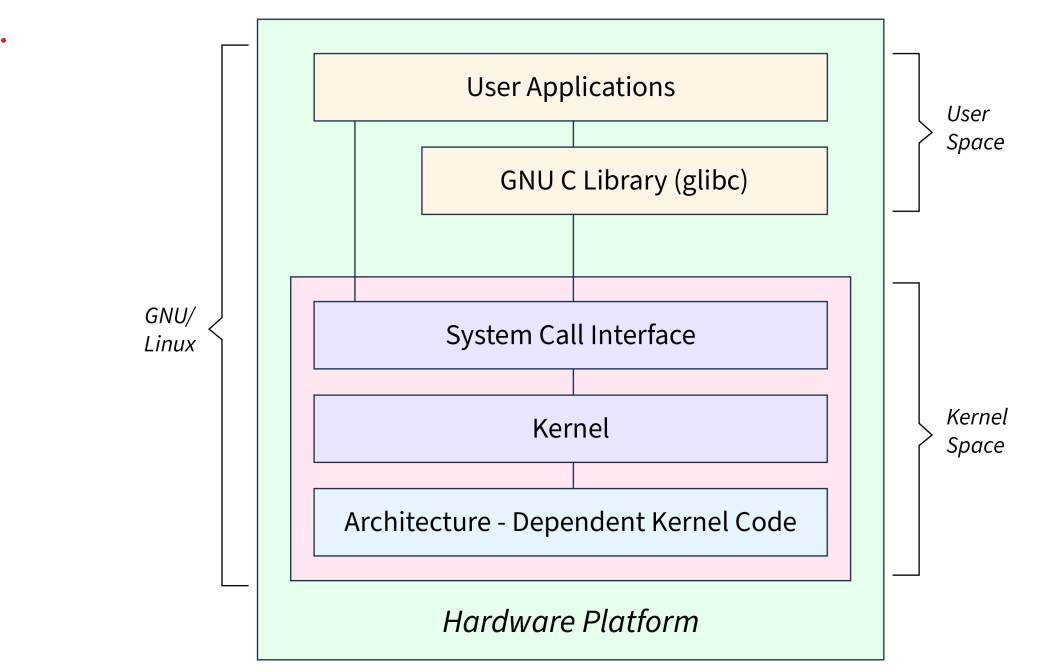
\includegraphics[width=0.9\linewidth]{"./images/arquitectura.png"}
		\caption{Esquema de la arquitectura del sistema GNU/Linux.}
		\label{fig:arquitectura}
	\end{figure}
	
	\subsubsection*{Espacio del kernel}
	
	\emph{Kernel:} es el programa central del sistema, inicia por el boot loader que es el encargado de las interacciones basicas del hardware con el sistema, ya sean tareas de lectura y escritura en disco duro, memoria RAM, controlares de dispositivos, asi como proporcionar un entorno virtual para iniciar las aplicaciones.
	\\
	\\
	\emph{Subsistemas:} son los programas que vienen instalados de manera predeterminada en el sistema, que se encargan de gestionar el acceso remoto, tener un bus central de mensajes/notificaciones y ejecutan acciones basadas en eventos de hardware o red.
	\\
	\\
	\emph{Herramienta de linea de comandos:} son programas pequeños que se ejecutan dentro de la linea de comandos o emulador de terminal, son capaces de editar texto, descargar archivos o administración del sistema.
	\\
	\\
	\emph{Inter Process Communication:} se encarga de tener una comunicación entre el kernel y las aplicaciones, por medio de un segmento compartido de memoria o un pequeño canal de comunicación creado por las aplicaciones para intercambio de datos. Otro método es a través del bus central de mensajes donde hay un intercambio de mensajes para comunicar todo el sistema. 
	
	\subsubsection*{Espacio del usuario}
	\emph{Librerías GNU:} son programas pequeños que controlar las ventanas, gráficos o lectura/escritura de las aplicaciones. Están desarrolladas en lenguaje C y cada una de ellas puede tener mas librerías para poder ser utilizada.
	\\
	\\
	\emph{Aplicaciones:} son todos aquellos programas finales, con los que el usuario puede interactuar con el sistema. Entre ellos están los navegadores web, editores de texto, reproductores de video o sonido, visualizadores de imágenes/videos, editores de imagen/video, entre muchos otros mas.
	
	\subsection*{¿Qué es una distribución?}
	Son configuraciones del kernel dependiendo de las necesidades de cierta comunidad, donde incluye una amplia gama de software, herramientas GNU, bibliotecas, interfaz grafica y aplicaciones. Cuenta con un administrador de paquetes para instalar, actualizar y eliminar software de manera sencilla. Algunas de las distribuciones mas populares son las siguientes:
	\\
	\\
	\emph{Ubuntu:} la mas popular por su facilidad de uso, documentación y soporte comunitario. Esta basado en Debian, lanzando cada seis meses nuevas versiones. Cuenta con versiones para escritorio, servers y cloud.	
	\begin{figure}[H]
		\centering
		
\includegraphics[width=0.3\linewidth]{"./images/ubuntu.png"}
		\caption{Logotipo distribución Ubuntu.}
		\label{fig:logoUbuntu}
	\end{figure}

	\emph{Linux Mint:} enfocado en brindar una experiencia completa lista para usar al incluir complementos de navegador, codecs multimedia y soporte para reproducción de DVD.	
	\begin{figure}[H]
		\centering
		
\includegraphics[width=0.3\linewidth]{"./images/mint.png"}
		\caption{Logotipo distribución Linux Mint.}
		\label{fig:logoMint}
	\end{figure}
	
	\emph{Fedora:} es patrocinado por Red Hat y es utilizado como distribución para su versión de empresa Red Hat Enterprise Linux. 
	\begin{figure}[H]
		\centering
		
\includegraphics[width=0.2\linewidth]{"./images/fedora.png"}
		\caption{Logotipo distribución Fedora.}
		\label{fig:logoFedora}
	\end{figure}
	
	\emph{Debian:} es una de las mas antiguas, estable, seguridad y amplios repositorios de software. Utiliza una amplia gama de arquitecturas y ofrece más $59,000$ paquetes de software, ademas de utilizar la gestión de paquetes con APT y su formato con extensión deb.
	\begin{figure}[H]
		\centering
		
\includegraphics[width=0.3\linewidth]{"./images/debian.png"}
		\caption{Logotipo distribución Debian.}
		\label{fig:logoDebian}
	\end{figure}
	
	\emph{Arch Linux:} dirigido a usuarios mas experimentados, siguiendo un modelo de lanzamiento continuo ofreciendo las ultimas versiones manteniendo la simplicidad y personalización. Utiliza pacman como administrador de paquetes y es conocido por una documentación completa y detallada.
	\begin{figure}[H]
		\centering
		
\includegraphics[width=0.3\linewidth]{"./images/arch.png"}
		\caption{Logotipo distribución Arch Linux.}
		\label{fig:logoArch}
	\end{figure}
	
	\subsection*{Comparativa}
	
	\section*{Comandos de navegación}
	\emph{ls:}
	\\
	\emph{cd:}
	\\
	\emph{pwd}
	\\
	\emph{whoami:}
	\\
	\emph{find:}
	
	\subsection*{Manipulación de ficheros}
	\emph{mkdir:}
	\\
	\emph{rmdir:}
	\\
	\emph{rm:}
	\\
	\emph{cp:} este comando permite copiar ficheros en el mismo directorio o subdirectorio.
	\\
	\\
	\begin{tabular}{|c|p{8cm}|}
		\hline
		Comando & Descripción \\
		\hline
		cp nombreFichero rutaDestino & copia el fichero en el directorio de destino con el mismo nombre del fichero de origen \\
		\hline
		cp nombreFichero1 nombreFichero2 & copia los ficheros que están separados por espacio en el directorio de destino con sus mismos nombres de origen \\
		\hline
		cp nombreFichero rutaDestino/nuevoNombre & copia el fichero de origen en el directorio de destino, pero con un nombre diferente \\
		\hline
		cp nombreFichero nuevoFichero & se copia el contenido del fichero de origen con un nuevo nombre en el mismo directorio \\
		\hline
		cp -a nombreFichero rutaDestino & se copia el fichero con los mismos permisos y metadatos que vienen asociados a el \\
		\hline
		cp -b nombreFichero rutaDestino & crea una copia en el buffer, los ficheros tienen el mismo nombre pero diferente contenido \\
		\hline
		cp -d nombreFichero rutaDestino & copia los enlaces simbólicos que se asocian al fichero \\
		\hline
		cp -f nombreFichero rutaDestino & sobrescribe el fichero al momento de copiar \\
		\hline
		cp -i nombreFichero rutaDestino & muestra un mensaje de advertencia antes de sobrescribir, acepta como respuesta y (si) y n (no) \\
		\hline
		cp -l nombreFichero rutaDestino & crea un enlace duro en vez de una copia \\
		\hline
		cp -n nombreFichero rutaDestino & los ficheros existentes no se sobrescriben \\
		\hline
		cp -p nombreFichero rutaDestino & se heredan todos los atributos del fichero original \\
		\hline
		cp -P nombreFichero rutaDestino & se guardan los enlaces simbólicos del fichero al copiar \\
		\hline
		cp -r directorioOrigen directorioDestino & copia de manera recursiva el contenido de uno o varios directorios en otro fichero, este fichero de destino no existe lo crea \\
		\hline
		cp -s nombreFichero rutaDestino & crea un enlace simbolico para el fichero original \\
		\hline
		cp -S nombreFichero rutaDestino & sobrescribe el backup del fichero \\
		cp -u nombreFichero rutaDestino & se copia el fichero si y solo si el fichero de origen es mas antiguo que el de destino \\
		\hline
		cp -v nombreFichero rutaDestino & emite un mensaje de alerta cuando termina el proceso \\
		\hline
	\end{tabular}
	\\
	\\
	\emph{mv:} con este comando se pueden mover ficheros y directorios
	\\
	\\
	\begin{tabular}{|p{7cm}|p{7cm}|}
		\hline
		Comando & Descripción \\
		\hline
		mv nombreFichero/nombreDirectorio directorioDestino & mueve ficheros o directorios a un directorio destino \\
		\hline
		mv -f nombreFichero/nombreDirectorio directorioDestino & mueve ficheros o directorios forzar la sobrescritura \\
		\hline
		mv -i nombreFichero/nombreDirectorio directorioDestino & antes de mover ficheros o directorios, pregunta si se desea sobrescribir \\
		\hline
		mv -u nombreFichero/nombreDirectorio directorioDestino & mueve ficheros o directorios, si y solo si el origen es mas antiguo que el destino \\
		\hline
		mv -v nombreFichero/nombreDirectorio directorioDestino & manda un mensaje al terminar el proceso \\
		\hline
		mv nombreFichero/nombreDirectorio nuevoNombreFichero/nuevoNombreDirectorio & cambia el nombre del archivo de origen \\
		\hline
		mv ER directorioDestino & mueve todo aquello que coincida con la expresión regular dada a un directorio destino \\
		\hline
		mv -b nombreFichero/nombreDirectorio directorioDestino & antes de mover el fichero o directorio, realiza una copia de seguridad, siempre y cuando exista el origen \\
		\hline
	\end{tabular}
	\\
	\\
	\emph{touch:}
	
	\section*{Visualización de texto}
	\emph{cat:} nos proporciona una interfaz sencilla para administración de ficheros de texto.
	\\ 
	\\
	\begin{tabular}{|p{7cm}|p{7cm}|}
		\hline
		Comando & Descripción \\
		\hline
		cat nombreFichero & muestra el contenido del fichero en la terminal \\
		\hline
		cat > nombreFichero & crea o sobrescribe un fichero, se habilita un cursor para introducir texto, al finalizar colocar la combinación de teclas Ctrl + d \\
		\hline
		cat >> nombreFichero & habilita un cursor para introducir texto a un fichero existente, al finalizar colocar la combinación de teclas Ctrl + d \\
		\hline
		cat -n nombreFichero & muestra el contenido con el numero de linea del lado izquierdo \\
		\hline
		cat -b nombreFichero & muestra el numero de linea solo a las que no están vacías \\
		\hline
		cat nombrefIchero > nuevoFichero & genera un fichero nuevo desde otro ya existente \\
		\hline
		cat nombreFichero nombreFichero > nuevoFichero & genera un fichero nuevo combinando dos o mas ficheros \\
		\hline
		cat -s nombreFichero & muestra el contenido eliminando la mayor parte de lineas vacias \\
		\hline
		cat -E nombreFichero & muestra los finales de linea con el simbolo \$ \\
		\hline
		cat -T nombreFichero & muestra las tabulaciones con el simbolo \textasciicircum I \\
		\hline
	\end{tabular}
	\\
	\\
	\emph{less:} muestra el texto de un fichero en la terminal, se activa con el comando "less nombreFichero".
	\\
	\\
	\begin{tabular}{|c|p{8cm}|}
		\hline
		Opción & Descripción \\
		\hline
		-c & limpia pantalla \\
		\hline
		+n & inicia el archivo desde la linea n \\
		\hline
		:p & si existe un fichero anterior en el buffer, se puede examinar \\
		\hline
		:d & elimina del buffer el fichero actual \\
		\hline
		e & navegación linea por linea \\
		\hline
		-S & deshabilita el auto ajuste de lineas \\
		\hline
		-g & resalta la coincidencia actual \\
		\hline
		-M & muestra datos de navegación del fichero \\
		\hline
		ng & Salta a la linea numero n \\
		\hline
		= & proporciona información del fichero \\
		\hline
		q & salir del entorno \\
		\hline
	\end{tabular}
	\\
	\\
	\emph{more:} muestra contenido de texto de un fichero, pero en un sistema de paginación, donde se desplaza pagina por pagina el contenido.
	\\
	\\
	\begin{tabular}{|c|p{8cm}|}
		\hline
		Comando & Descripción \\
		\hline
		more nombreFichero & se abre el fichero correspondiente \\
		\hline
		more nombreFichero nombreFichero & apertura de mas de un fichero \\
		\hline
		more -n nombreFichero & al abrir muestra el numero de linea del lado izquierdo \\
		\hline
		more -valor nombreFichero & muestra un numero especifico de lineas \\
		\hline
		more +/[ER] & se abre el fichero en la primera coincidencia \\
		\hline
	\end{tabular}
	\emph{echo:} este comando sirve para imprimir texto o variables en la terminal
	\\
	\\
	\begin{tabular}{|c|p{8cm}|}
		\hline
		Comando & Descripción \\
		\hline
		echo "texto" & imprime el texto que esta dentro de las comillas \\
		\hline
		echo \$variable & imprime el contenido de la variable especificada \\
		\hline
		echo -e "caracterEscape" & tiene como salida la acción del carácter de escape que se tiene como argumento \\
		\hline
	\end{tabular}
	\\
	Dentro de las opciones de caracteres de escape se tienen los siguientes:
	\\
	\\
	\begin{tabular}{|c|p{8cm}|}
		\hline
		Opción & descripción \\
		\hline
		\textbackslash a & emite un sonido de alerta \\
		\hline
		\textbackslash c & suprime el salto de texto \\
		\hline
		\textbackslash n & salto de linea \\
		\hline
		\textbackslash r & vuelve al inicio de la linea \\
		\hline
		\textbackslash t & realiza una tabulación horizontal \\
		\hline
		\textbackslash v & realiza una tabulación vertical \\
		\hline
		\textbackslash \textbackslash & imprime la barra invertida \\
		\hline
	\end{tabular}
	\\
	\\
	\emph{grep:} busca información en base a patrones o expresiones regulares
	\\
	\\
	\begin{tabular}{|c|p{7cm}|}
		\hline
		Comando & Descripción \\
		\hline
		grep patron nombreFichero & busca el patrón especificado en el fichero \\
		\hline
		grep patron nombreFichero nombreFichero & busca el patrón especificado en dos o mas ficheros, los nombres tienen que ir separados por un espacio \\
		\hline
		grep -w patron nombreFichero & si coincide el patrón de búsqueda regresa un True \\
		\hline
		grep -i patron nombreFichero & busca el patrón deshabilitando sensitive case, no distingue mayúsculas y minúsculas \\
		\hline
		grep -c patron nombreFichero & devuelve el numero coincidencias en el texto \\
		\hline
		grep -v patron nombreFichero & omite las lineas de coincidencia \\
		grep -n patron nombreFichero & si encuentra coincidencias muestra el numero de la linea donde se encontró \\
		\hline
		grep -L patron & busca el patron en los ficheros del directorio actual y si encuentra coincidencias, muestra el nombre del Fichero \\
		\hline
		grep -e expresionRegular & busca la expresión regular en el Fichero \\
		\hline
		grep -e expresionRegular -e expresionRegular & búsqueda de varias expresiones regulares en el fichero \\
		\hline
	\end{tabular}
	\\
	\\
	El comando grep como se muestra en la tabla es capaz de realizar por medio de expresiones regulares, estas son patrones no específicos que pueden ser construidos, conforme a cierto criterio, para realizar búsquedas complejas con pocos caracteres de búsqueda. Pueden consultar mas información en el siguiente enlace https://tinyurl.com/24g3hzpk
	\\
	\\

	\section*{Compresión y descompresión}
	La compresión de ficheros o directorios nos es util cuando queremos enviar, subir o descargar una gran cantidad de información pero sin tener el tamaño completo, por lo que se ocupan comandos para comprimir y reducir esta cantidad a un poco mas accesible.
	\\
	\\
	tar nombreFichero.tar.gz directorio/fichero
	\\
	\\
	\begin{tabular}{|c|p{8cm}|}
		\hline
		Opción & Descripción \\
		\hline
		-z & comprime un fichero o directorio usando gzip \\
		\hline
		-c & crear un nuevo archivo \\
		\hline
		-v & muestra el porcentaje del proceso de comprensión \\
		\hline
		-f & nombre del fichero \\
		\hline
	\end{tabular}
	\\
	\\
	gzip -n nombreFichero
	\\
	\\
	\begin{tabular}{|c|p{8cm}|}
		\hline
		Opción & Descripción \\
		\hline
		-n & valor del 1 al 9, significa el nivel de compresión que debe tener el archivo final \\
		\hline
	\end{tabular}
	\\
	\\
	zip nombreFichero.zip fichero/directorio
	\\
	\\
	rar -a nombreFichero.rar fichero/directorio
	\\
	\\
	Una vez teniendo un fichero o directorio comprimido se puede distribuir para su uso, pero no es posible utilizarlo de manera directa, ya que el formato con el que este comprimido en ocasiones no es posible acceder a estos ficheros, por lo que se utilizan comandos de descompresión como los siguientes:
	\\
	\\
	tar -xvzf nombreFichero.tar.gz
	\\
	\\
	\begin{tabular}{|c|p{8cm}|}
		\hline
		Opción & Descripción \\
		\hline
		-x & extrae el contenido del fichero comprimido \\
		\hline
		-v & muestra el porcentaje del proceso de descompresión \\
		\hline
		-f & nombre del fichero \\
		\hline
	\end{tabular}
	\\
	\\
	gzip -d nombreFichero.gz o bzip2 -d nombreFichero.bz2
	\\
	\\
	\begin{tabular}{|c|p{8cm}|}
		\hline
		Opción & Descripción \\
		\hline
		-d & descompresión del fichero \\
		\hline
	\end{tabular}
	\\
	\\
	unzip nombreFichero.zip
	\\
	\\
	rar -x nombreFichero.rar
	\\
	\\
	\begin{tabular}{|c|p{8cm}|}
		\hline
		Opción & Descripción \\
		\hline
		-x & extrae el contenido del fichero comprimido \\
		\hline
	\end{tabular}
	
	\section*{Administración}
	
	\section*{Permisos}
	\emph{chmod:} este comando a su traducción al español seria cambio de modo, nos proporciona el cambio de permisos tanto a ficheros, asi como a directorios.
	\\
	Para realizar cambio se utilizan las siguientes clases usuario (u), grupo (g), otros (o) y todas las clases (a), a su vez se tienen tres permisos importantes que con lectura (r), escritura (w) y ejecución (x). Entonces para poder asignar estos permisos a los ficheros o directorios se tienen los siguientes operadores:
	\\
	\\
	\begin{tabular}{|c|p{8cm}|}
		\hline
		Operador & Descripción \\
		\hline
		+ & asigna permisos a la clase correspondiente \\
		\hline
		- & elimina permisos a la clase correspondiente \\
		\hline
		= & se renuevan los permisos, sin importar los que se tenían antes \\
		\hline
	\end{tabular}
	\\
	\\
	También es posible utilizar una combinación de números para colocar permisos, la sintaxis para poder hacerlo es a través de una cantidad de tres dígitos donde cada uno representa la clase con respecto al sistema ugo. En la siguiente tabla se muestra la combinación de permisos, conforme a la numeración en binario del 0 al 7:
	\\
	\\
	\begin{tabular}{|c|c|c|c|c|}
		\hline
		r & w & x & decimal & Permiso \\
		\hline
		0 & 0 & 0 & 0 & ningun permiso \\
		\hline
		0 & 0 & 1 & 1 & solo ejecución \\
		\hline
		0 & 1 & 0 & 2 & solo escritura \\
		\hline
		0 & 1 & 1 & 3 & ejecución y escritura \\
		\hline
		1 & 0 & 0 & 4 & solo lectura \\
		\hline
		1 & 0 & 1 & 5 & lectura y ejecución \\
		\hline
		1 & 1 & 0 & 6 & lectura y escritura \\
		\hline
		1 & 1 & 1 & 7 & todos los permisos \\
		\hline
	\end{tabular}
	\\
	\\
	Existen opciones para el comando, las cuales son:
	\\
	\\
	\begin{tabular}{|c|p{8cm}|}
		\hline
		Opción & Descripción \\
		\hline
		-R & modifica los permisos de forma recursiva para todos los ficheros y subdirectorios del directorio principal \\
		\hline
		-v & después de terminar la ejecución se realiza el diagnostico de los ficheros procesados \\
		\hline
		-c & después de terminar la ejecución muestra un diagnostico para los ficheros modificados \\ 
		\hline
		-f & no muestra los mensajes de error \\
		\hline
	\end{tabular}
	\\
	\\
	\emph{chown y chgrp:} ambos comandos funcionan de manera similar con la diferencia en el tipo de cambio que realizan, chown cambiar le nombre de propietario/grupo, mientras que chgrp solo cambia el grupo. Para ambos casos bastan con proporcionan el nombre o el ID asociado al propietario o grupo.
	\\
	\\
	\begin{tabular}{|p{7cm}|p{7cm}|}
		\hline
		Comando & Descripción \\
		\hline
		chown nombrePropietario nombreFichero & cambia el propietario del fichero \\
		\hline
		chown nombrePropietario nombreDirectorio & cambia el propietario del directorio \\
		\hline
		chown nombrePropietario:nombreGrupo nombreFichero/Directorio & cambia el propietario y el grupo del fichero o directorio \\
		\hline
		chgrp nombreGrupo nombreFichero/Directorio & cambia el grupo del fichero o directorio \\
		\hline
	\end{tabular}
	
	
	\section*{Networking}
	\emph{Ping:} se utiliza para saber el estado de las interfaces de red instaladas en nuestro equipo, si hay un envió de paquetes quiere decir que tenemos una conexión fuera de nuestro entorno local, si existe una perdida revisar que pasa con la interfaz. El resultado de este comando se divide en dos partes: la secuencia de envió individual por paquete y las estadísticas globales del comando.
	\\
	\\
	\emph{Información individual:} muestra el envió de paquetes uno a uno.
	\\
	\begin{tabular}{|c|p{8cm}|}
		\hline
		Atributo & Descripción \\
		\hline
		icmp\_seq & numero de la secuencia en el envió de paquetes para el Internet Control Message Protocol, este aumenta en 1 por cada paquete enviado, si existe un salto en la numeración nos indica un paquete perdido. \\
		\hline
		ttl(Time To Live) & es el número máximo de saltos que puede viajar el paquete antes de descartarse, por cada router visitado este valor disminuye en 1, si se llega a 0 se descarta el paquete y se envía un mensaje de error. \\
		\hline
		time (rtt) & tiempo de ida y vuelta que tarda un paquete en llegar al destino y volver, medido en milisegundos (ms) \\
		\hline
	\end{tabular}
	\\
	\\
	\emph{Información general:} estadísticas globales del proceso de envió para los paquetes, lleva el nombre de rtt(Round Trip Time)
	\\
	\\
	\begin{tabular}{|c|p{8cm}|}
		\hline
		Atributo & Descripción \\
		\hline
		packets transmitted & número total de paquetes enviados por ICMP \\
		\hline
		received & número de paquetes recibidos \\
		\hline
		packet loss (\%) & porcentaje de paquetes perdidos en la transmisión \\
		\hline
		time (ms) & tiempo total transcurrido de la prueba de ping \\
		\hline
		min & menor tiempo de envió y recepción \\
		\hline
		max & máximo tiempo de envió y recepción \\
		\hline
		avg & tiempo promedio del envió y recepción de todos los paquetes \\
		\hline
		mdev & desviación estándar nos indica que tanto varían los tiempos de envió, si el valor es pequeño hay una conexión estable y un valor grande es una red inestable \\
		\hline
	\end{tabular}
	\\
	\\
	\emph{Opciones para el comando ping}
	\\
	\\
	\begin{tabular}{|c|p{8cm}|}
		\hline
		Comando & Descripción \\
		\hline
		ping IP/host & realiza un envió de paquetes en bucle hasta terminar el proceso \\
		\hline
		ping localhost & realiza un ping de manera local \\
		\hline
		ping -c n IP/host & hace un envió de n paquetes  \\
		\hline
		ping -i n IP/host & envía los paquetes en el intervalo de cada n segundos  \\
		\hline
		ping -f IP/host & envía los paquetes lo mas rápido que permite la interfaz de red, si se cuenta con un limite de velocidad este comando no realiza nada y manda un mensaje \\
		\hline
		ping -s n IP/host & cambia el tamaño de Bytes de los paquetes a enviar \\
		\hline
		ping -q IP/host & realiza el ping y al finalizar solo muestra la información de resumen \\
		\hline
		ping -w n IP/host & se detiene el envió de paquetes pasados n segundos \\
		\hline
	\end{tabular}
	\\
	\\
	\emph{ifconfig:} es una herramienta de gestión de red, utilizada para configurar y ver el estado de las interfaces que se encuentran conectadas en nuestro equipo, este paquete esta deprecado para versiones nuevas por lo que se necesita instalar.
	\\
	\\
	Para poder obtener el paquete para su uso se tiene el siguiente comando sudo apt-get install net-tools -y, la opción -y nos indica que aceptara la instalación sin pausar la instalación para preguntar, otro punto importante es que este comando debe ser utilizado en modo superusuario.
	\\
	\\
	\begin{tabular}{|c|p{7cm}|}
		\hline
		Comando & Descripción \\
		\hline
		ifconfig -a & muestra la información de las interfaces conectadas y las ip asociadas a ella \\
		\hline
		ifconfig nombreInterfaz & muestra la información de la interfaz de red del nombre que se paso como argumento \\
		\hline
		ifconfig nombreInterfaz IP netmask mascaraRed & asigna la IP y mascara de red a la interfaz dada como parámetro \\
		\hline
		ifconfig nombreInterfaz down & deshabilita la interfaz de red que se da como parámetro \\
		\hline
		ifconfig nombreInterfaz up & habilita la interfaz de red que se da como parámetro \\
		\hline
		ifconfig nombreInterfaz mtu valorMTU & limita el tamaño de transferencia de paquetes para esa interfaz \\
		\hline
		ifconfig nombreInterfaz hw ether MAC & cambia la dirección MAC de la interfaz de red \\
		\hline
	\end{tabular}
	\\
	\\
	\emph{ip:} sustituye a ifconfig, por lo que es mas potente para gestionar interfaces de red. Este paquete no necesita ser instalado y tampoco ser utilizado con superusuario.
	\\
	\\
	\begin{tabular}{|p{8cm}|p{7cm}|}
		\hline
		Comando & Descripción \\
		\hline
		ip adrr & muestra toda la información de las interfaces de red conectadas en nuestro equipo, así como las ip asociadas a cada una \\
		\hline
		ip link show & ver y gestionar, se enfoca en el estado físico de las interfaces \\
		\hline
		ip link set dev nombreInterfaz down & deshabilita la interfaz de red dada como parámetro \\
		\hline
		ip link set dev nombreInterfaz up & habilita la interfaz de red dada como parámetro \\
		\hline
		ip route show & muestra las tablas de enrutamiento del sistema \\
		\hline
		ip route add IP/mascaraRED via IP & agrega una nueva ruta a la tabla de rutas del sistema \\
		\hline
		ip route del IP/mascaraRED via IP & elimina una ruta de la tabla de rutas del sistema \\
		\hline
		ip neigh show & muestra la tabla ARP IPv4 y la NDP IPv6. \\
		\hline
		ip tunnel [add/change/delete] nombreTunel mode [IPIP/sit/GRE] [remote/local/dev] IP & gestiona lo referente a túneles \\ 
		\hline
		ip adrr add IP/mascaraRed dev nombreTunel & asigna una IP a un túnel especifico \\
		\hline
	\end{tabular}
	\\
	\\
	en ip tunnel se tienen las siguientes opciones:

	\begin{itemize}
		\item IPIP: túnel de IP sobre IP
		\item sit: túneles para IPv6
		\item GRE: túneles para Cisco
	\end{itemize}

	\begin{itemize}
		\item remote: dirección de salida del túnel
		\item local: dirección local de entrada del túnel
		\item dev: nombre del periférico a través del que se envían los paquetes
	\end{itemize}
	
	\emph{netstat:} supervisa, diagnostica, y recopila datos de las diferentes interfaces de red.
	\\
	\\
	\begin{tabular}{|c|p{8cm}|}
		\hline
		Comando & Descripción \\
		\hline
		netstat -a & muestra todo, incluido sockets de escucha y no escucha \\
		\hline
		netstat -l & muestra solamente sockets de escucha \\
		\hline
		netstat -t & muestra conexiones TCP \\
		\hline
		netstat -u & muestra conexiones UDP \\
		\hline
		netstat -r & muestra la tabla de enrutamiento del sistema \\
		\hline
		netstat -pag & muestra el ID del proceso y nombre del rpograma asociado con cada conexión \\
		\hline
		netstat -norte & direcciones númericas en lugar de mostrar el nombre del host \\
		\hline
		netstat -s & muestra estadísticas para protocolos de transferencia de paquetes \\
		\hline
		netstat -i & muestra las interfaces de red del equipo, asi como sus estadisticas \\
		\hline
	\end{tabular}
	\\
	\\
	\emph{curl:} sirve para poder enviar datos por petición HTTP/HTTPS, gestionar APIs, asi como subir o descargar archivos por servidor ftp.
	\\
	\\
	\begin{tabular}{|p{7cm}|p{7cm}|}
		\hline
		Comando & Descripción \\
		\hline
		curl url & muestra la respuesta del servidor, normalmente contenido HTML \\
		\hline
		curl -o nombreArchivo url & guarda la respuesta en un archivo \\
		\hline
		curl -L url & realiza un seguimiento de todo el sitio \\
		\hline
		curl -d '{"json":"data"}' url & envía datos en formato json \\
		\hline
		curl -H "Header: valor" url & envía cabeceras HTTP personalizadas \\
		\hline
		curl -X [POST, GET, PUT, PATCH, DELETE] url & utiliza cualquier método HTTP \\
		\hline
		curl -s url & modo silencioso, no muestra barra de progreso \\
		\hline
		curl -S url & muestra mensajes de error aunque este activo el modo silencioso \\
		\hline
		curl -v url & muestra cabeceras enviadas y recibidas \\
		\hline
		curl -u user:password url & inicio de sesión básico \\
		\hline
		curl -u user:password ftp://url/htdocs & lista los archivos en el servidor \\
		\hline
		curl -u user:password ftp://url/htdocs/ruta -o nombreArchivo & descarga un archivo desde el servidor \\
		\hline
		curl -T nombreArchivo -u user:password ftp://url/htdocs & realiza una subida del archivo correspondiente al servidor \\
		\hline
		curl -T nombreArchivo -u user:password ftp://url/htdocs/ruta & realiza la subida del archivo correspondiente en una carpeta especifica \\
		\hline
	\end{tabular}
	\\
	\\
	\emph{wget:} realiza descargas de archivos específicos o sitios completos.
	\\
	\\
	\begin{tabular}{|c|p{8cm}|}
		\hline
		Comando & Descripción \\
		\hline
		wget url/archivo & descarga un archivo \\
		\hline
		wget -P ruta url/archivo & descarga un archivo en una ruta especifica \\
		\hline
		wget -b url/archivo & realiza la descarga en segundo plano, sin mostrar nada en el proceso, solo al finalizar \\
		\hline
		wget -c url/archivo & si se detiene la descarga se puede reanudar \\
		\hline
		wget --limit-rate:valor url/archivo & limita la velocidad de descarga \\
		\hline
		wget url/archivo url/archivo \\ wget -i archivo.txt & descarga varios archivos \\
		\hline
	\end{tabular}
	\\
	\\
	Para realizar la descarga de un sitio completo se tiene el siguiente comando:
	\\
	\\
	wget --recursive --no-clobber --page-requisites --html-extension --convert-links --restrict-file-name=windows --domains dominio --no-parent url
	\\
	\\
	Donde se tiene la siguiente tabla con la descripción para cada opción:
	\\
	\\
	\begin{tabular}{|c|p{8cm}|}
		\hline
		Opción & Descripción \\
		\hline
		- -recursive & descarga el sitio siguiendo todas las rutas internas \\
		\hline
		- -no-cobbler & no sobrescribe ningún archivo \\
		\hline 
		- -page-requisites & obtiene todos los elementos del sitio \\
		\hline
		- -html-extension & guarda los archivos con extensión html \\
		\hline
		- -convert-links & conversión de enlaces para funcionamiento completo \\
		\hline
		- -restrict-file-name=windows & modifica los archivos para que puedan funcionar en el sistema operativo windows \\
		\hline
		--domains dominio & no sigue nada fuera del dominio especificado \\
		\hline
		--no-parent & no sigue enlaces fuera del directorio principal del dominio \\
		\hline
	\end{tabular}
	
	\section*{Principales directorios en Linux}
	Dentro de cualquier distribución basada en el kernel de Linux, tenemos un sistema de archivos el cual contiene directorios específicos para el funcionamiento del sistema operativo, la siguiente tabla menciona los directoios que se utilizan con mayor frecuencia.
	\\
	\\
	\begin{tabular}{|c|p{9cm}|}
		\hline
		Directorio & Descripción \\
		\hline
		/bin & ficheros binarios para ejecución de las aplicaciones del sistema \\
		\hline
		/etc & contiene los ficheros de configuración y scripts de arranque del sistema \\
		\hline
		/home & contiene los directorios personales para cada usuarios, algunos de ellos son descargas, escritorio, imagenes, entre otros \\
		\hline
		/var & ficheros con variables de registro y bases de datos \\
		\hline
		/usr & contiene los ficheros que puede tener acceso un usuario, así como aplicaciones \\
		\hline
		/tmp & guarda ficheros temporales que necesitan las aplicaciones para instalaciones, configuraciones u otro motivo \\
		\hline
		/root & contiene los directorios del superusuario, los cuales tienen aplicaciones, configuraciones usuarios, scripts de arranque, ficheros del kernel \\
		\hline
	\end{tabular}
	\\
	\\
	Para poder acceder a estos directorios basta con utilizar el comando cd y mandar como argumento el nombre del directorio a acceder, teniendo en cuento colocar / al inicio del nombre.
	
	\section*{Referencias}
	FYCGROUP. UNIX: La simplicidad del ingenio, fyccorp.com consultado el 17 de agosto de 2025, recuperado de https://fyccorp.com/unix-la-simplicidad-del-ingenio/	
	\\
	\\
	GNU. ¿Qué es GNU?, www.gnu.org, consultado el 17 de agosto de 2025, recuperado de https://www.gnu.org/home.es.html
	\\
	\\
	Floriano, J.(2024). ¿Qué es el sistema Linux y cuáles son sus ventajas?, BlogSEAS, consultado el 17 de agosto de 2025, recuperado de https://www.seas.es/blog/informatica/que-es-el-sistema-linux-y-cuales-son-sus-ventajas/
	\\
	\\
	Denisse. (2016). Una mirada dentro del núcleo de Linux, lignux.com, consultado el 18 de agosto de 2025, recuperado de https://lignux.com/una-mirada-dentro-del-nucleo-linux/
	\\
	\\
	Spasojevic, A. (2024). ¿Qué es una distribución de Linux?, phoenixnap.mx, consultado el 18 de agosto de 2025, recuperado de https://phoenixnap.mx/glosario/que-es-una-distribucion-de-linux
	
\end{document}